\chapter{Data \label{ch:data}}
In this chapter the necessary data for the calibration of the sensors is presented. Section \ref{sec:da:vector_fields} explains what information about the fields is used to calibrate the sensors. Section \ref{sec:da:calibration_meas} presents the calibration measurement which was done. 


\begin{wrapfigure}{r}{0.27\linewidth}
    \centering
    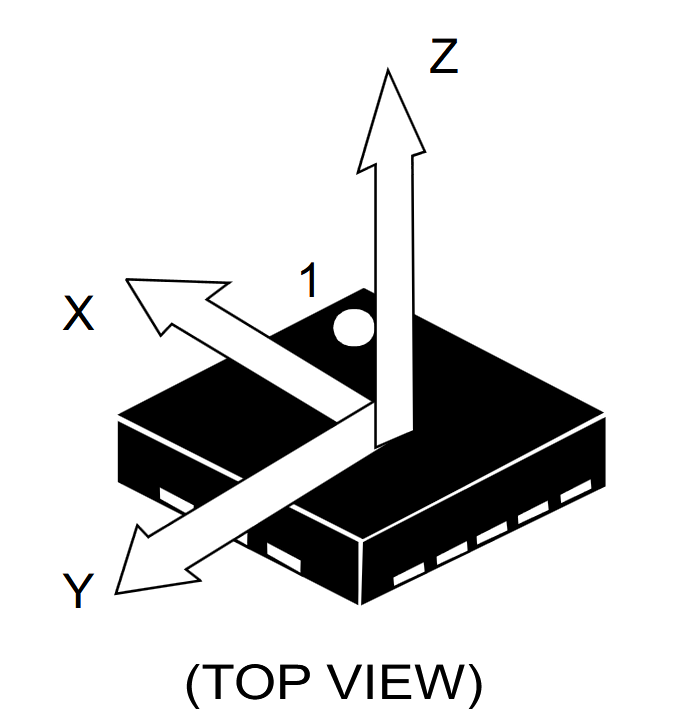
\includegraphics[width=\linewidth]{images/03_data/chip_coord_sys.png}
    \caption{Coordinate system of the accelerometer.}
    \label{fig:data:chip_coord_sys}
\end{wrapfigure}
The intrinsic coordinate system of the accelerometer chip is shown in fig. \ref{fig:data:chip_coord_sys}. The sensor measures the acceleration of the proof mass relative to the substrate which is connected rigidly with the device housing. When the sensor is laying on the table and no forces are applied to it, the sensor will read an acceleration value of +1$g$ on the z-axis. The table on which the sensor lays exerts a force onto the housing, and thus the substrate, antiparallel and of the same magnitude as the gravitational force. This normal force is measured by the accelerometer. The gravity vector is the only acceleration we are interested in, so we change the sign of the z-axis' measurement value to align the gravity vector with the negative z-axis (compare fig. \ref{fig:body_frame}). The same problem applies to the measurement of the x- and y-axis. To circumnavigate it, the axes of the chip (fig. \ref{fig:data:chip_coord_sys}) are mirrored to generate the body frame of measurement presented in fig. \ref{fig:body_frame}. The body frame coordinate system is still right-handed, just like fig. manual, because two of the three axes were reinterpreted.

The x- and y-axes of the magnetometer are multiplied by $-1$ to realign the magnetometers coordinate system with the body frame.

%If the sensor is accelerated to the left (e.g. positive x axis), because of Newton's first law of motion the proof mass swings to the right. The output reads a positive acceleration in x direction. If the sensor box is laid down with chip z to zenith, a positive value is registered, because the sensor acts as if it was accelerated upwards and the mass is "dangling" downward because of Newton I. The corrected coordinate system should be positive z to the zenith and a right-hand coordinate system. Ideally we would just mirror all three chip axes to get our new coordinate system. This works very well with the x and y axes. When laying the chip on its port side the output reads 1. The chip interprets the proof mass being accelerated port side as the chip as a whole being accelerated to starboard which it displays as a +1 on the y axis. We would now like to interpret this in the corrected coordinate system that +1 g on the y axis is pointing downwards. Thus the number value will stay the same and only the interpretation is changed. Same for the x axis. As the zenith axes of the chip and correct system should align pointing upwards, we will simply multiply the measured value by -1. If the chip is laying with chip z upwards, the proof mass is deflected downwards with 1g  which is equivalent to an acceleration of the sensor as a whole of +1g upwards (because the sensor works with inertia), which is displayed. We would however very much like to interpret this +1g of acceleration as -1g because the gravity vector is defined as $ (0, 0, -g)^T $. \\
%In short: x and y axis are simply reinterpreted and because z cannot be reinterpreted it is multiplied by $-1$.

\begin{figure}[H]
    \centering
    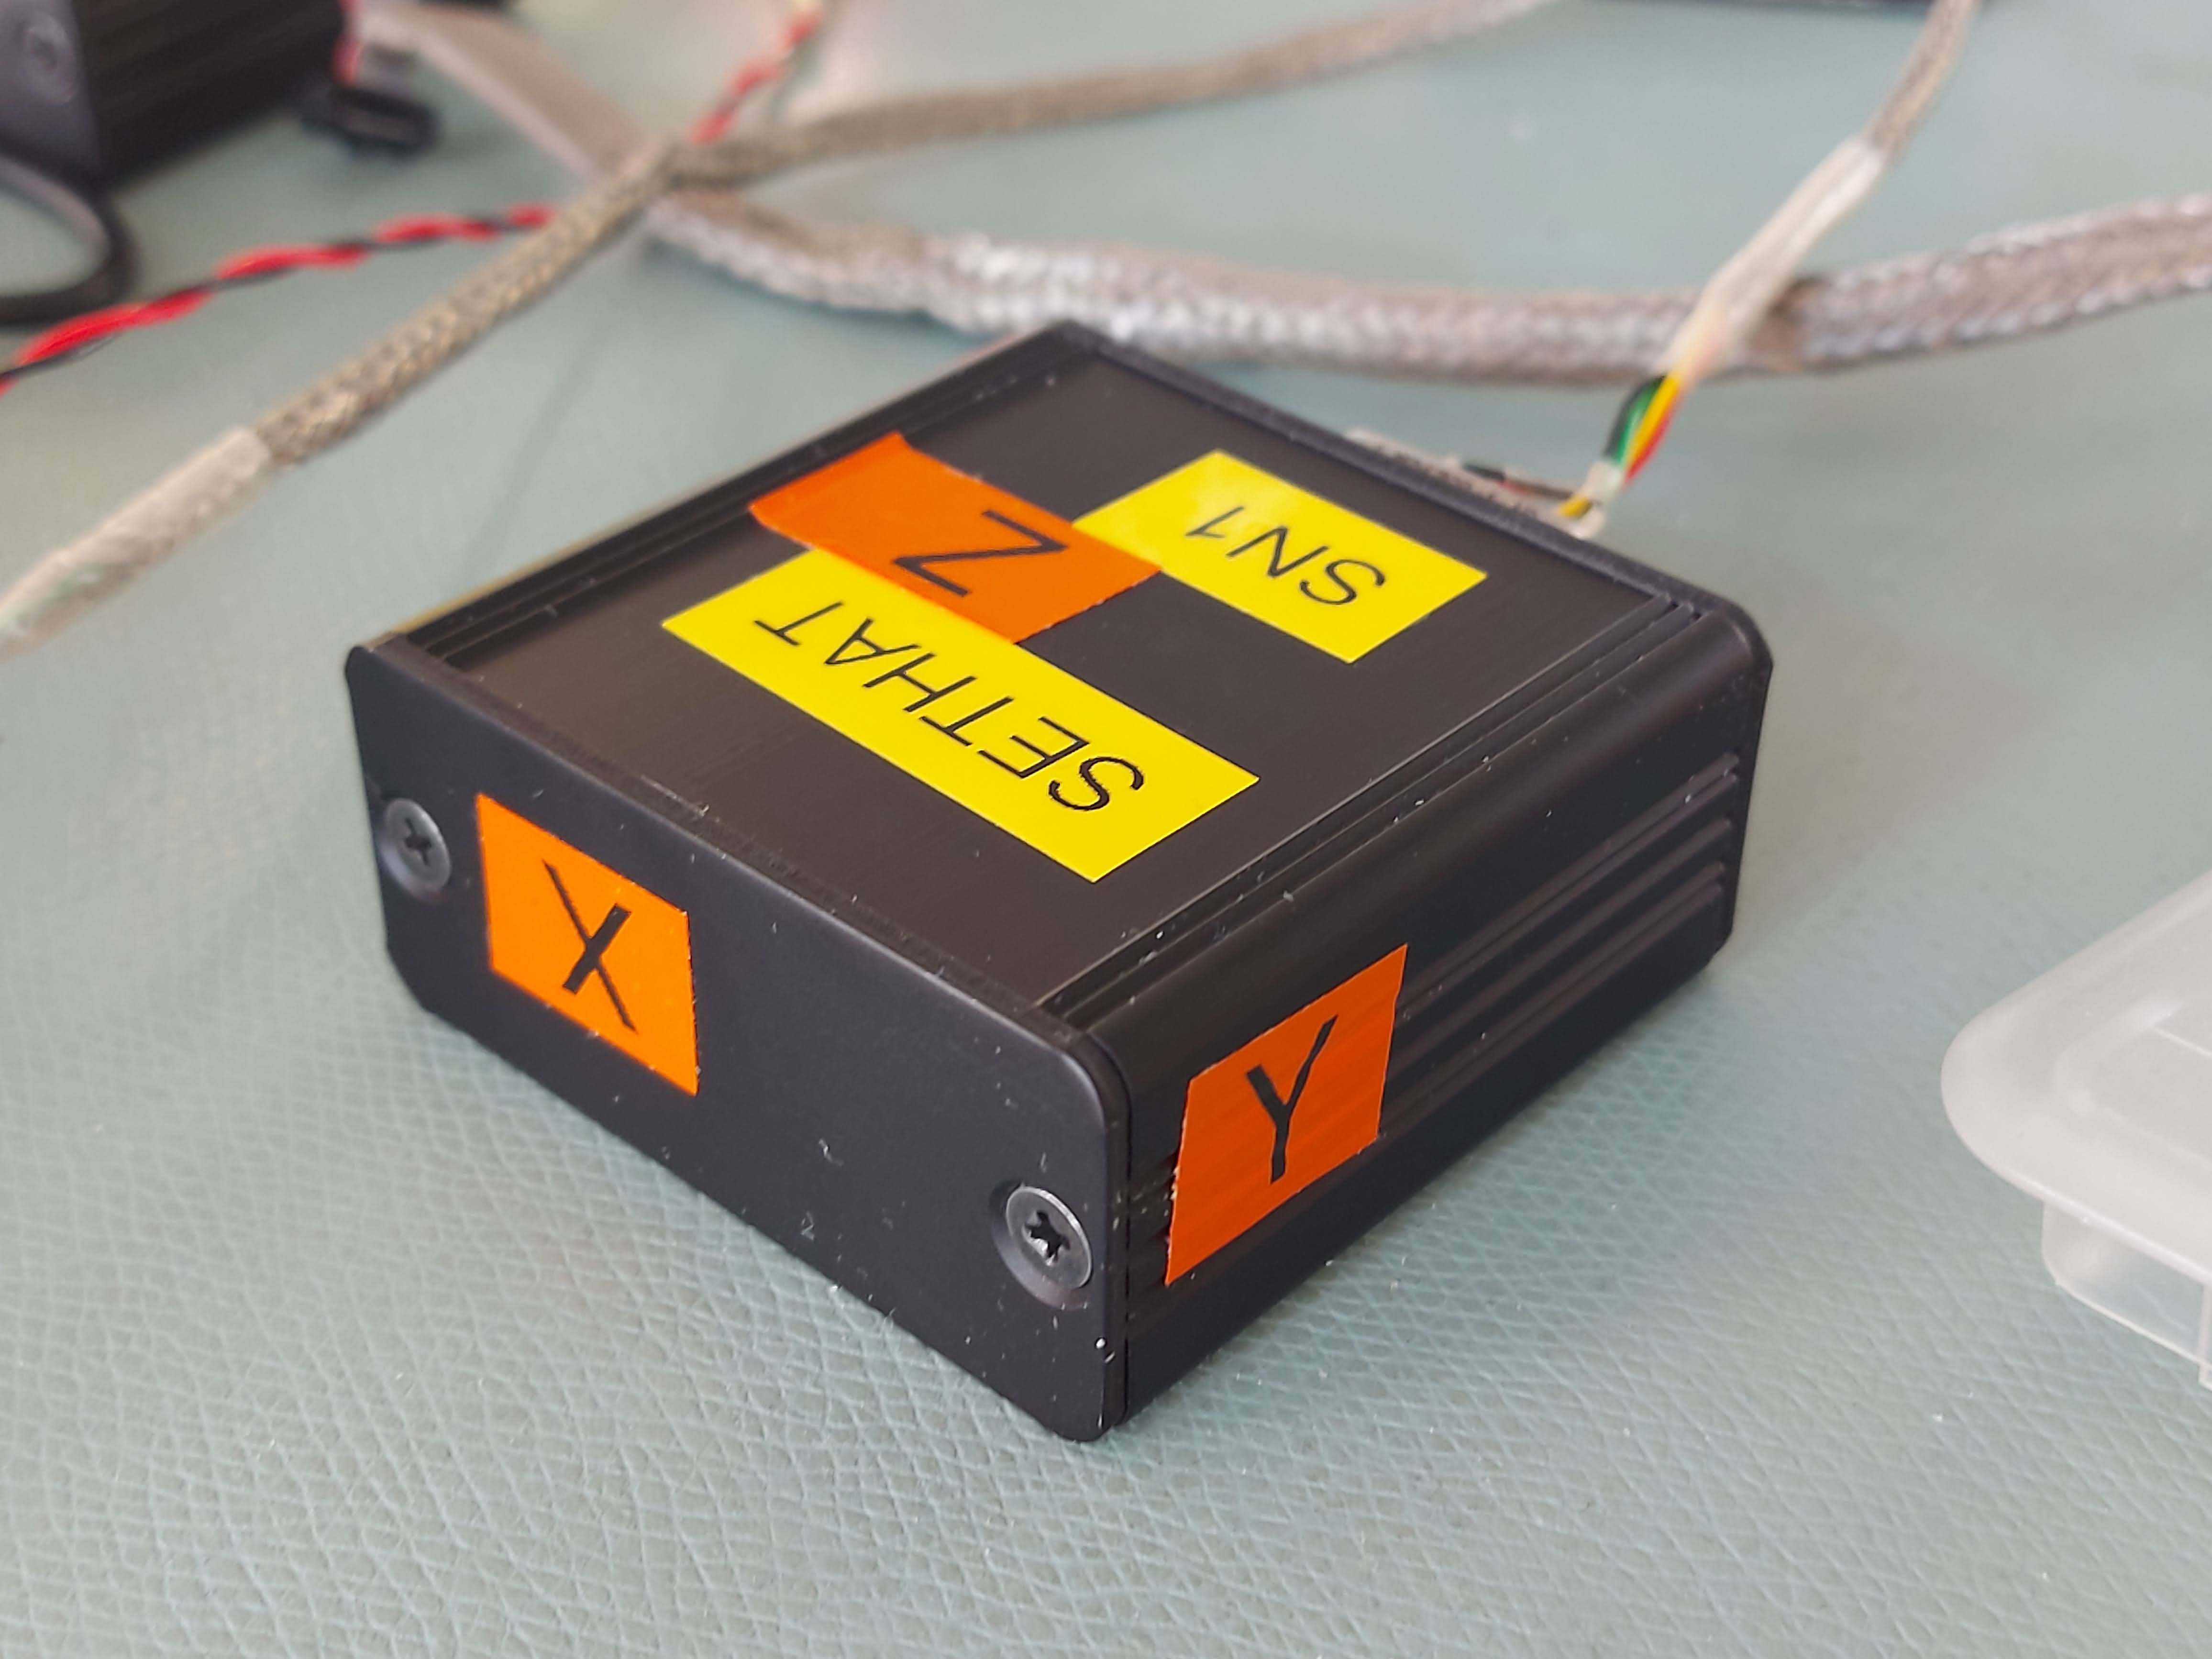
\includegraphics[width=0.8\linewidth]{images/03_data/ads_sensor_axes.jpg}
    \caption{Axes of the \ac{ADS} sensor.}
    \label{fig:body_frame}
\end{figure}

\section{Vector fields \label{sec:da:vector_fields}}
The \ac{DOC} \ac{NOAA} has publicly available geomagnetic field calculators using the \acf{WMM}, \acf{IGRF}, \acf{EMM} or \acf{WMMHR}. Because no uncertainty is provided for the \ac{IGRF} values and the \ac{EMM} is only valid for the years 2000 to 2019 both of these models are not considered. The \ac{WMM} and \ac{WMMHR} values for Kiel (54\deg\,20'\,18''\,N 10\deg\,7'34''\,E) on 1\:April\:2025 at 0\,km above \ac{MSL} are presented in table \ref{tab:da:mag_models_comp}.

\begin{table}[h]
    \centering
    \begin{tabular}{r|ccc}
        Model & \ac{WMM} & \ac{WMMHR} & \ac{WMMHR} at 40\,km \ac{MSL}\\\hline
        Declination & 4\deg\,9'\,35''\,E & 4\deg\,12'\,27''\,E & 4\deg\,5'\,27''\,E \\
        North Comp. (mGs) & 177.8(1.4) & 178.4(1.4) & 175.6(1.4) \\ 
        East Comp. (mGs) & 12.9(0.9) & 13.1(0.9) & 12.6(0.9) \\
        Vertical Comp. (mGs) & 470.0(1.4) & 470.5(1.3) & 461.7(1.3) \\
        Total Field (mGs) & 502.6(1.4) & 503.4(1.3) & 494.2(1.3) \\
    \end{tabular}
    \caption[Comparison of the \acs{WMM} \parencite{WMM} and \acs{WMMHR} \parencite{WMMHR} in Kiel.]{Comparison of the \acs{WMM} \parencite{WMM} and \acs{WMMHR} \parencite{WMMHR}. Given in brackets are the uncertainties. All values are rounded to the error.}
    \label{tab:da:mag_models_comp}
\end{table}

Because of its lower uncertainties in all components of the magnetic field the \ac{WMMHR} is chosen for the calibration of the magnetometer.\\
As the difference between 0\,km and 40\,km above \ac{MSL} is non-negligible at 10\,mGs, the different values will be used when applicable. When fitting the ground based measurement, the value for 0\,km altitude ($(503.4\,\mathrm{mGs})^2=0.25341156\mathrm{(Gs)}^2$) is used and when fitting the flight, the value for 40\,km altitude ($(494.2\,\mathrm{mGs})^2=0.24423364\mathrm{(Gs)}^2$) is used.

The Accelerometer returns values in units of $g$, thus the magnitude of the field used for calibration is simply 1.

\section{Calibration Measurement \label{sec:da:calibration_meas}}
To find the coefficients $a$, $b$, $c$, $x_0$, $y_0$ and $z_0$ a calibration measurement is taken in the \ac{IEAP}'s courtyard/car park on 11 April 2025. Figure \ref{fig:test_lab} shows the area where the measurements are taken in red. To measure outside of the home electronics laboratory, the Ethernet is disconnected and the power pins are connected to four AA 1.5\,V batteries. The lab setup is shown in fig. \ref{fig:ads_mobile} without the battery pack and with Ethernet connected. The \ac{ADS} resides in the black box marked with "SETHAT" "SN1". 

\begin{figure}[h]
    \begin{subfigure}[t]{.5\textwidth}
        \centering
        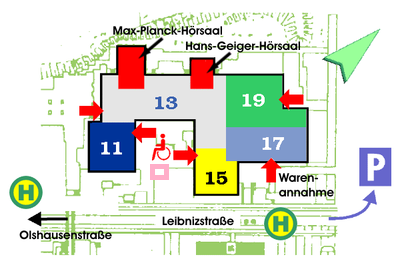
\includegraphics[width=0.9\linewidth]{images/03_data/lageplan Physikzentrum.png}
        \caption[Floor plan of the Physikzentrum.]{Floor plan of the Physikzentrum. Marked in pink is the area shown in \ref{fig:test_lab}.}
        \label{fig:lageplan_physikzentrum}
    \end{subfigure}
    \begin{subfigure}[t]{.5\textwidth}
    \centering
    \includegraphics[width=0.9\linewidth]{images/03_data/calibration_test_lab.jpg}
    \caption[Test laboratory for the calibration measurement.]{Test laboratory for the calibration measurement. Marked in red is the area where measurements were taken.}
    \label{fig:test_lab}
    \end{subfigure}
    \caption{Location of the calibration measurement.}
\end{figure}

\begin{figure}[h]
    \centering
    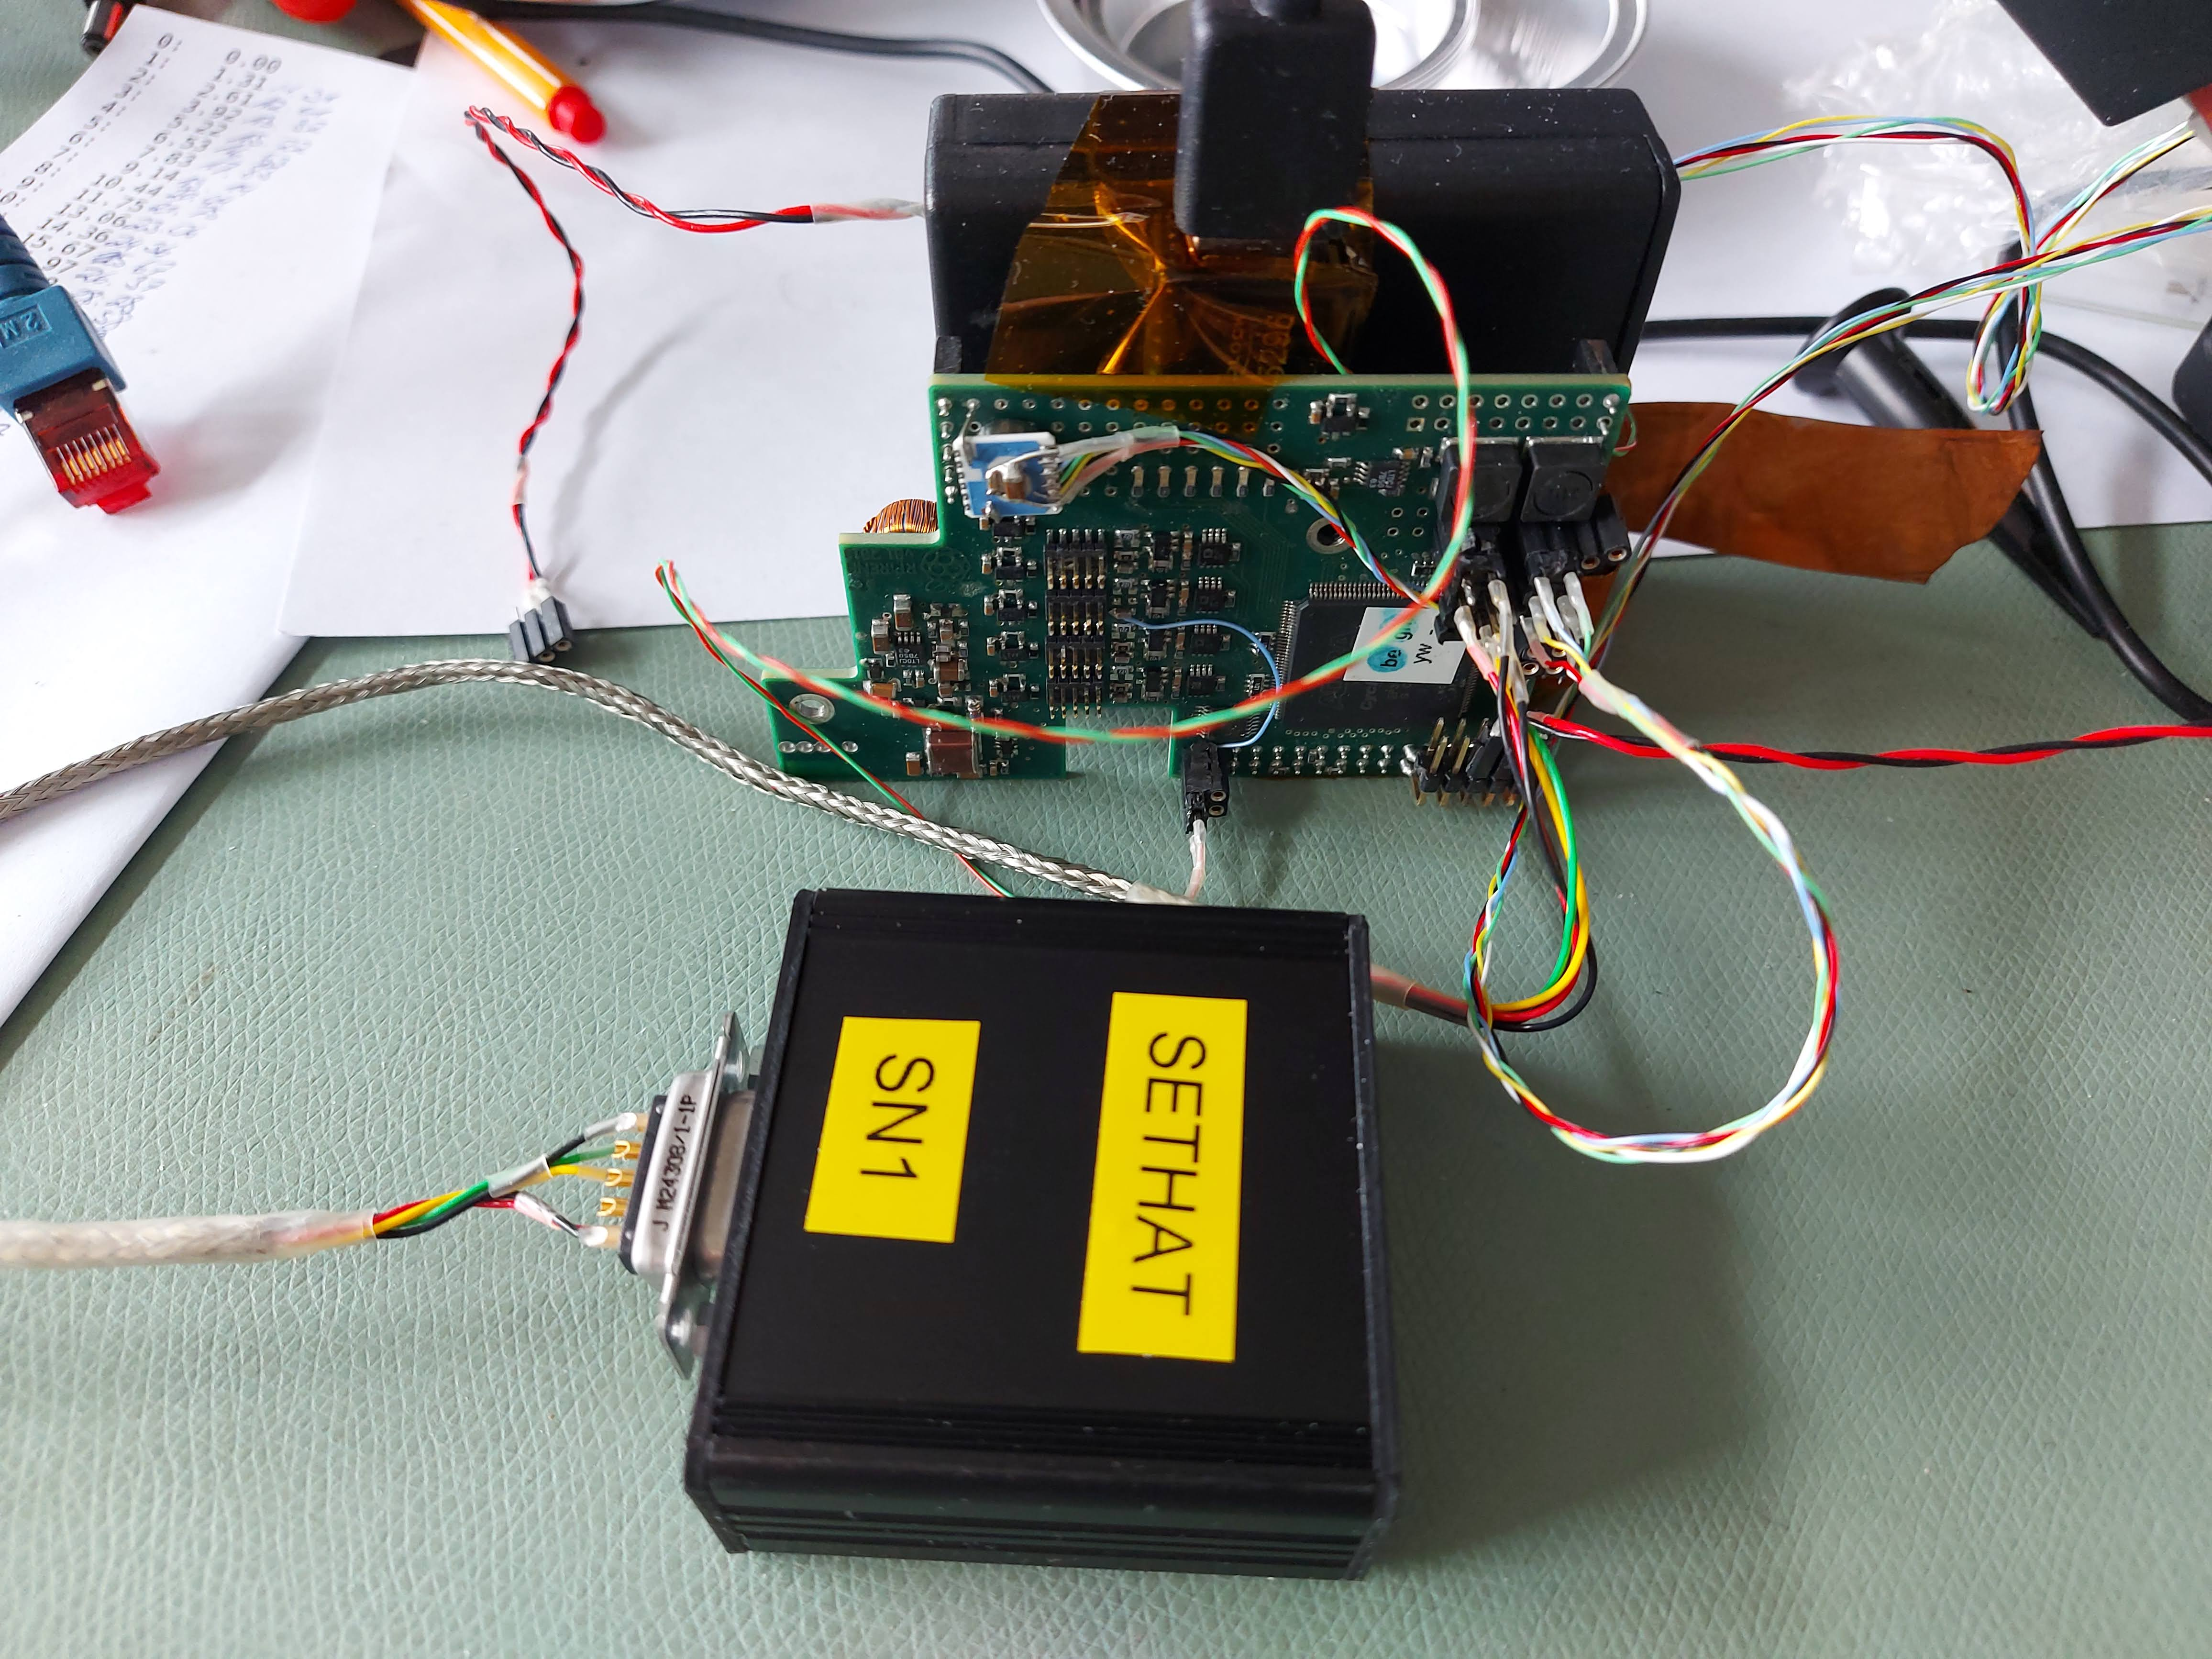
\includegraphics[width=0.7\linewidth]{images/03_data/sethat_mobile.jpg}
    \caption{Mobile version of the \ac{ADS}.}
    \label{fig:ads_mobile}
\end{figure}